\section{Representação de grafos}

\begin{frame}[fragile]{Matriz de adjacências}

    \begin{itemize}
        \item Seja $N = |V|$ e considere que cada vértice $v\in V$ é representado por um
            número positivo distinto do intervalo $[1, N]$

        \item A representação de um grafo por matriz de adjacências utiliza uma matriz
            $A_{N\times N}$, onde o elemento $a_{ij}$ armazena o peso da aresta que une o vértice
            $i$ ao vértice $j$

        \item Em um grafo não-ponderado, $a_{ij} = 1$ representa a existência da aresta, e 
            $a_{ij} = 0$ a inexistência da mesma

        \item Outra interpretação possível é considerar $a_{ij}$ o número de ocorrências da aresta
            $(i, j)$ em um multigrafo não-ponderado

        \item Em um grafo simples, $a_{ii} = 0, \forall i\in V$

        \item Esta representação responde perguntas do tipo ``Há uma aresta entre $u$ e $v$? Qual
            é o seu peso?'' em $O(1)$

        \item Contudo, a complexidade de memória é alta ($O(N^2)$)
    \end{itemize}

\end{frame}

\begin{frame}[fragile]{Visualização da representação por matriz de adjacências}

    \begin{figure}
        \centering

        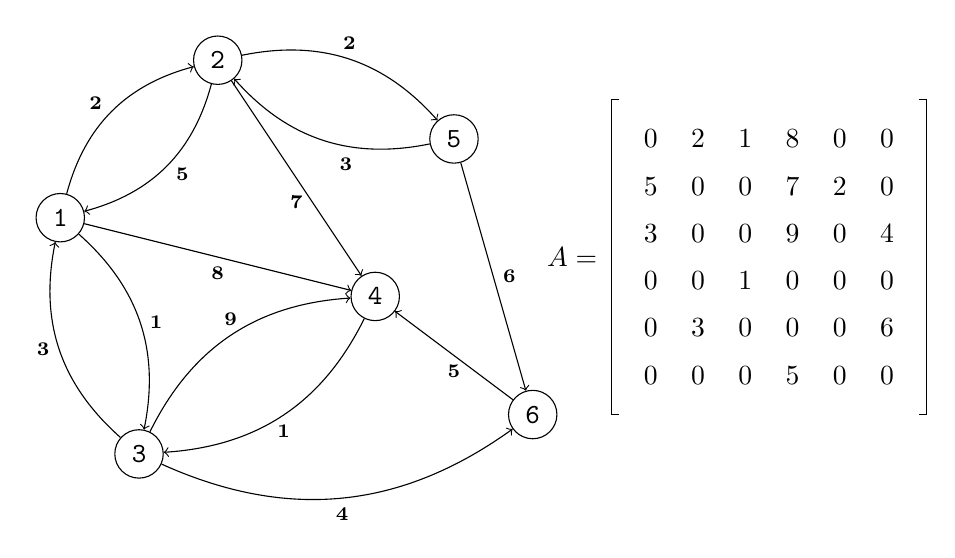
\begin{tikzpicture}
            \node[draw,circle] (A) at (0, 3) { \tt 1 };
            \node[draw,circle] (B) at (2, 5) { \tt 2 };
            \node[draw,circle] (C) at (1, 0) { \tt 3 };
            \node[draw,circle] (D) at (4, 2) { \tt 4 };
            \node[draw,circle] (E) at (5, 4) { \tt 5 };
            \node[draw,circle] (F) at (6, 0.5) { \tt 6 };

            \draw[->] (A) to [bend left] node[anchor=east,yshift=0.1cm] { \scriptsize $\mathbf{2}$ } (B);
            \draw[->] (B) to [bend left] node[anchor=west,yshift=-0.1cm] { \scriptsize $\mathbf{5}$ } (A);
            \draw[->] (A) to [bend left] node[anchor=west] { \scriptsize $\mathbf{1}$ } (C);
            \draw[->] (C) to [bend left] node[anchor=east] { \scriptsize $\mathbf{3}$ } (A);
            \draw[->] (D) to [bend left] node[anchor=north] { \scriptsize $\mathbf{1}$ } (C);
            \draw[->] (C) to [bend left] node[anchor=south] { \scriptsize $\mathbf{9}$ } (D);
            \draw[->] (B) to [bend left] node[anchor=south] { \scriptsize $\mathbf{2}$ } (E);
            \draw[->] (E) to [bend left] node[anchor=north,xshift=0.3cm,yshift=-0.1cm] { \scriptsize $\mathbf{3}$ } (B);

            \draw[->] (A) -- node[anchor=north] { \scriptsize $\mathbf{8}$ } (D);
            \draw[->] (B) -- node[anchor=north,yshift=-0.1cm] { \scriptsize $\mathbf{7}$ } (D);
            \draw[->] (C) to [bend right] node[anchor=north] { \scriptsize $\mathbf{4}$ } (F);
            \draw[<-] (D) -- node[anchor=north] { \scriptsize $\mathbf{5}$ } (F);
            \draw[->] (E) -- node[anchor=west] { \scriptsize $\mathbf{6}$ } (F);

            \node at (6.5, 2.5) { $A = $ };
            \draw (7.1, 4.5) -- (7, 4.5) -- (7, 0.5) -- (7.1, 0.5);
            \draw (10.9, 4.5) -- (11, 4.5) -- (11, 0.5) -- (10.9, 0.5);

            \node at (7.5, 4) { $0$ };
            \node at (8.1, 4) { $2$ };
            \node at (8.7, 4) { $1$ };
            \node at (9.3, 4) { $8$ };
            \node at (9.9, 4) { $0$ };
            \node at (10.5, 4) { $0$ };

            \node at (7.5, 3.4) { $5$ };
            \node at (8.1, 3.4) { $0$ };
            \node at (8.7, 3.4) { $0$ };
            \node at (9.3, 3.4) { $7$ };
            \node at (9.9, 3.4) { $2$ };
            \node at (10.5, 3.4) { $0$ };

            \node at (7.5, 2.8) { $3$ };
            \node at (8.1, 2.8) { $0$ };
            \node at (8.7, 2.8) { $0$ };
            \node at (9.3, 2.8) { $9$ };
            \node at (9.9, 2.8) { $0$ };
            \node at (10.5, 2.8) { $4$ };

            \node at (7.5, 2.2) { $0$ };
            \node at (8.1, 2.2) { $0$ };
            \node at (8.7, 2.2) { $1$ };
            \node at (9.3, 2.2) { $0$ };
            \node at (9.9, 2.2) { $0$ };
            \node at (10.5, 2.2) { $0$ };

            \node at (7.5, 1.6) { $0$ };
            \node at (8.1, 1.6) { $3$ };
            \node at (8.7, 1.6) { $0$ };
            \node at (9.3, 1.6) { $0$ };
            \node at (9.9, 1.6) { $0$ };
            \node at (10.5, 1.6) { $6$ };

            \node at (7.5, 1.0) { $0$ };
            \node at (8.1, 1.0) { $0$ };
            \node at (8.7, 1.0) { $0$ };
            \node at (9.3, 1.0) { $5$ };
            \node at (9.9, 1.0) { $0$ };
            \node at (10.5, 1.0) { $0$ };

        \end{tikzpicture}

    \end{figure}

\end{frame}


\begin{frame}[fragile]{Representação por matriz de adjacências}
    \inputsnippet{cpp}{1}{21}{matriz.cpp}
\end{frame}

\begin{frame}[fragile]{Representação por lista de adjacências}

    \begin{itemize}
        \item Na representação por lista de adjacências, a cada vértice $u$ é associada uma lista
            que contém os identificadores dos vértices $v$ relacionados a $u$

        \item Caso o grafo seja ponderado, cada entrada da lista contém duas informações: o 
            identificador do vértice $v$ e o peso $w$ da aresta $(u, v)$

        \item Em C++, estas listas podem ser contêniers do tipo \code{c}{list}, \code{c}{vector}
            ou \code{c}{forward_list}

        \item A escolha depende do tipo de travessia que será feita em cada aresta que parte de $u$

        \item Esta representação é mais adequada para grafos esparsos do que as matrizes de 
            adjacência, uma vez que tem complexidade de memória $O(N + M)$

        \item A maioria dos algoritmos clássicos de grafos utiliza esta representação
    \end{itemize}

\end{frame}

\input{listas_view}

\begin{frame}[fragile]{Representação por lista de adjacências}
    \inputsnippet{cpp}{1}{21}{listas.cpp}
\end{frame}

\begin{frame}[fragile]{Representação por lista de arestas}

    \begin{itemize}
        \item Na representação por lista de arestas o grafo é representado pelo conjunto $E$
            das arestas

        \item Se o grafo é ponderado, cada aresta corresponderá a uma tripla com os valores
            $(u, v, w)$, que indica que a aresta $(u, v)$ tem peso $w$

        \item Observe que é possível obter o conjunto $V$ a partir de $E$ caso o grafo $G(V, E)$
            não possua vértices isolados

        \item Esta representação tem complexidade $O(M)$, onde $M = |E|$

        \item Esta representação é utilizada no algoritmo de Kruskall para árvore mínima 
            geradora

        \item Nos demais algoritmos a implementação pode ficar mais trabalhosa, ou mesmo
            ter maior complexidade assintótica, uma vez que os vértices $V$ não podem ser
            acessados diretamente
    \end{itemize}

\end{frame}

\begin{frame}[fragile]{Visualização da representação por lista de arestas}

    \begin{figure}
        \centering

        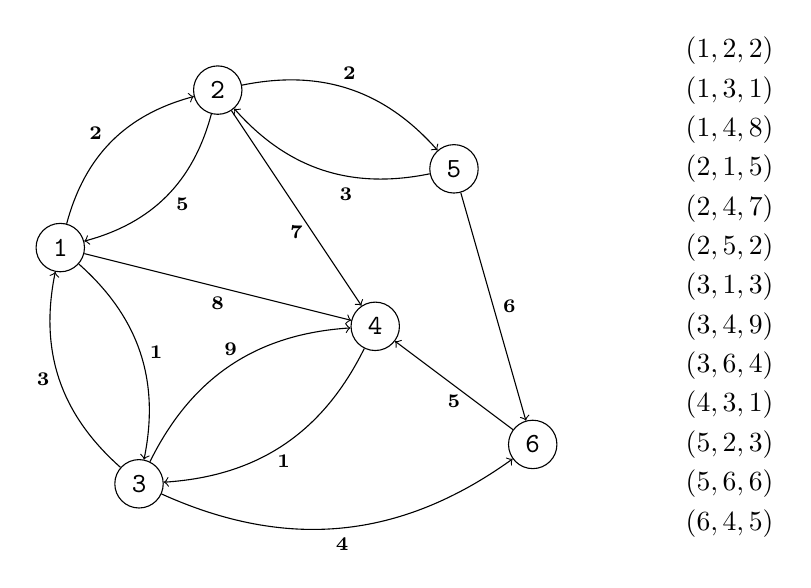
\begin{tikzpicture}
            \node[draw,circle] (A) at (0, 3) { \tt 1 };
            \node[draw,circle] (B) at (2, 5) { \tt 2 };
            \node[draw,circle] (C) at (1, 0) { \tt 3 };
            \node[draw,circle] (D) at (4, 2) { \tt 4 };
            \node[draw,circle] (E) at (5, 4) { \tt 5 };
            \node[draw,circle] (F) at (6, 0.5) { \tt 6 };

            \draw[->] (A) to [bend left] node[anchor=east,yshift=0.1cm] { \scriptsize $\mathbf{2}$ } (B);
            \draw[->] (B) to [bend left] node[anchor=west,yshift=-0.1cm] { \scriptsize $\mathbf{5}$ } (A);
            \draw[->] (A) to [bend left] node[anchor=west] { \scriptsize $\mathbf{1}$ } (C);
            \draw[->] (C) to [bend left] node[anchor=east] { \scriptsize $\mathbf{3}$ } (A);
            \draw[->] (D) to [bend left] node[anchor=north] { \scriptsize $\mathbf{1}$ } (C);
            \draw[->] (C) to [bend left] node[anchor=south] { \scriptsize $\mathbf{9}$ } (D);
            \draw[->] (B) to [bend left] node[anchor=south] { \scriptsize $\mathbf{2}$ } (E);
            \draw[->] (E) to [bend left] node[anchor=north,xshift=0.3cm,yshift=-0.1cm] { \scriptsize $\mathbf{3}$ } (B);

            \draw[->] (A) -- node[anchor=north] { \scriptsize $\mathbf{8}$ } (D);
            \draw[->] (B) -- node[anchor=north,yshift=-0.1cm] { \scriptsize $\mathbf{7}$ } (D);
            \draw[->] (C) to [bend right] node[anchor=north] { \scriptsize $\mathbf{4}$ } (F);
            \draw[<-] (D) -- node[anchor=north] { \scriptsize $\mathbf{5}$ } (F);
            \draw[->] (E) -- node[anchor=west] { \scriptsize $\mathbf{6}$ } (F);

            \node at (8.5, 5.5) { $(1, 2, 2)$ };
            \node at (8.5, 5) { $(1, 3, 1)$ };
            \node at (8.5, 4.5) { $(1, 4, 8)$ };
            \node at (8.5, 4) { $(2, 1, 5)$ };
            \node at (8.5, 3.5) { $(2, 4, 7)$ };
            \node at (8.5, 3) { $(2, 5, 2)$ };
            \node at (8.5, 2.5) { $(3, 1, 3)$ };
            \node at (8.5, 2) { $(3, 4, 9)$ };
            \node at (8.5, 1.5) { $(3, 6, 4)$ };
            \node at (8.5, 1) { $(4, 3, 1)$ };
            \node at (8.5, 0.5) { $(5, 2, 3)$ };
            \node at (8.5, 0) { $(5, 6, 6)$ };
            \node at (8.5, -0.5) { $(6, 4, 5)$ };
        \end{tikzpicture}

    \end{figure}

\end{frame}


\begin{frame}[fragile]{Representação por lista de arestas}
    \inputsnippet{cpp}{1}{21}{arestas.cpp}
\end{frame}

\begin{frame}[fragile]{Representação implícita}

    \begin{itemize}
        \item Na representação implícita os vértices e arestas são dadas implicitamente, por 
            meio de relações matemáticas ou pelo contexto do problema

        \item Por exemplo, o grafo completo formado pelos pontos do plano cartesiano cujas 
            coordenadas são números inteiros, e cujos pesos das arestas são dados pela distância 
            euclidiana, é um grafo implícito

        \item Esta representação é adequada quando o grafo for muito complexo ou quando a 
            relação entre os vértices é óbvia ou diretamente computável

        \item Também pode ser utilizada para construir um grafo sob demanda, o que é útil em
            problemas de teoria dos jogos ou em simulações
    \end{itemize}

\end{frame}
